% !TeX spellcheck = pl_PL
%%%%%%%%%%%%%%%%%%%%%%%%%%%%%%%%%%%%%%%%%%%
%                                        %
% Szablon pracy dyplomowej inzynierskiej %
% zgodny  z aktualnymi  przepisami  SZJK %
%                                        %
%%%%%%%%%%%%%%%%%%%%%%%%%%%%%%%%%%%%%%%%%%
%                                        %
%  (c) Krzysztof Simiński, 2018-2023     %
%                                        %
%%%%%%%%%%%%%%%%%%%%%%%%%%%%%%%%%%%%%%%%%%
%                                        %
% Najnowsza wersja szablonów jest        %
% podstępna pod adresem                  %
% github.com/ksiminski/polsl-aei-theses  %
%                                        %
%%%%%%%%%%%%%%%%%%%%%%%%%%%%%%%%%%%%%%%%%%
%
%
% Projekt LaTeXowy zapewnia odpowiednie formatowanie pracy,
% zgodnie z wymaganiami Systemu zapewniania jakości kształcenia.
% Proszę nie zmieniać ustawień formatowania (np. fontu,
% marginesów, wytłuszczeń, kursywy itd. ).
%
% Projekt można kompilować na kilka sposobów.
%
% 1. kompilacja pdfLaTeX
%
% pdflatex main
% bibtex   main
% pdflatex main
% pdflatex main
%
%
% 2. kompilacja XeLaTeX
%
% Kompilatacja przy użyciu XeLaTeXa różni się tym, że na stronie
% tytułowej używany jest font Calibri. Wymaga to jego uprzedniego
% zainstalowania.
%
% xelatex main
% bibtex  main
% xelatex main
% xelatex main
%
%
%%%%%%%%%%%%%%%%%%%%%%%%%%%%%%%%%%%%%%%%%%%%%%%%%%%%%
% W przypadku pytań, uwag, proszę pisać na adres:   %
%      krzysztof.siminski(małpa)polsl.pl            %
%%%%%%%%%%%%%%%%%%%%%%%%%%%%%%%%%%%%%%%%%%%%%%%%%%%%%
%
% Chcemy ulepszać szablony LaTeXowe prac dyplomowych.
% Wypełniając ankietę spod poniższego adresu pomogą
% Państwo nam to zrobić. Ankieta jest całkowicie
% anonimowa. Dziękujemy!


% https://docs.google.com/forms/d/e/1FAIpQLScyllVxNKzKFHfILDfdbwC-jvT8YL0RSTFs-s27UGw9CKn-fQ/viewform?usp=sf_link
%
%%%%%%%%%%%%%%%%%%%%%%%%%%%%%%%%%%%%%%%%%%%%%%%%%%%%%%%%%%%%%%%%%%%%%%%%%

%%%%%%%%%%%%%%%%%%%%%%%%%%%%%%%%%%%%%%%%%%%%%%%
%                                             %
% PERSONALIZACJA PRACY – DANE PRACY           %
%                                             %
%%%%%%%%%%%%%%%%%%%%%%%%%%%%%%%%%%%%%%%%%%%%%%%

% Proszę wpisać swoje dane w poniższych definicjach.

% TODO
% dane autora
\newcommand{\FirstNameAuthor}{Łukasz}
\newcommand{\SurnameAuthor}{Grabarski}
\newcommand{\IdAuthor}{300434}   % numer albumu  (bez $\langle$ i $\rangle$)

% drugi autor:
%\newcommand{\FirstNameCoauthor}{Imię}   % Jeżeli jest drugi autor, to tutaj należy podać imię.
%\newcommand{\SurnameCoauthor}{Nazwisko} % Jeżeli jest drugi autor, to tutaj należy podać nazwisko.
%\newcommand{\IdCoauthor}{$\langle$wpisać właściwy$\rangle$}  % numer albumu drugiego autora (bez $\langle$ i $\rangle$)
% Gdy nie ma drugiego autora, należy zostawić poniższe definicje puste, jak poniżej. Gdy jest drugi autor, należy zakomentować te linie.
\newcommand{\FirstNameCoauthor}{} % Jeżeli praca ma tylko jednego autora, to dane drugiego autora zostają puste.
\newcommand{\SurnameCoauthor}{}   % Jeżeli praca ma tylko jednego autora, to dane drugiego autora zostają puste.
\newcommand{\IdCoauthor}{}  % Jeżeli praca ma tylko jednego autora, to dane drugiego autora zostają puste.
%%%%%%%%%%

\newcommand{\Supervisor}{dr inż. Krzysztof Jaskot}     % dane promotora (bez $\langle$ i $\rangle$)
\newcommand{\Title}{System wizyjny dla robota mobilnego}           % tytuł pracy po polsku
\newcommand{\TitleAlt}{Vision system for a mobile robot}                     % thesis title in English
\newcommand{\Program}{Automatyka i Robotyka}            % kierunek studiów  (bez $\langle$ i $\rangle$)
\newcommand{\Specialisation}{Technologie Informacyjne}     % specjalność  (bez $\langle$ i $\rangle$)
\newcommand{\Departament}{Automatyki i Robotyki}        % katedra promotora  (bez $\langle$ i $\rangle$)

% Jeżeli został wyznaczony promotor pomocniczy lub opiekun, proszę go/ją wpisać ...
\newcommand{\Consultant}{} % dane promotora pomocniczego, opiekuna (bez $\langle$ i $\rangle$)
% ... w przeciwnym razie proszę zostawić puste miejsce jak poniżej:
%\newcommand{\Consultant}{} % brak promotowa pomocniczego / opiekuna

% koniec fragmentu do modyfikacji
%%%%%%%%%%%%%%%%%%%%%%%%%%%%%%%%%%%%%%%%%%


%%%%%%%%%%%%%%%%%%%%%%%%%%%%%%%%%%%%%%%%%%%%%%%
%                                             %
% KONIEC PERSONALIZACJI PRACY                 %
%                                             %
%%%%%%%%%%%%%%%%%%%%%%%%%%%%%%%%%%%%%%%%%%%%%%%

%%%%%%%%%%%%%%%%%%%%%%%%%%%%%%%%%%%%%%%%


%%%%%%%%%%%%%%%%%%%%%%%%%%%%%%%%%%%%%%%%%%%%%%%
%                                             %
% PROSZĘ NIE MODYFIKOWAĆ PONIŻSZYCH USTAWIEŃ! %
%                                             %
%%%%%%%%%%%%%%%%%%%%%%%%%%%%%%%%%%%%%%%%%%%%%%%



\documentclass[a4paper,twoside,12pt]{book}
\usepackage[utf8]{inputenc}                                      
\usepackage[T1]{fontenc}  
\usepackage{amsmath,amsfonts,amssymb,amsthm}
\usepackage[british,polish]{babel} 
\usepackage{indentfirst}
\usepackage{xurl}
\usepackage{xstring}
\usepackage{ifthen}



\usepackage{ifxetex}

\ifxetex
	\usepackage{fontspec}
	\defaultfontfeatures{Mapping=tex—text} % to support TeX conventions like ``——-''
	\usepackage{xunicode} % Unicode support for LaTeX character names (accents, European chars, etc)
	\usepackage{xltxtra} % Extra customizations for XeLaTeX
\else
	\usepackage{lmodern}
\fi



\usepackage[margin=2.5cm]{geometry}
\usepackage{graphicx} 
\usepackage{hyperref}
\usepackage{booktabs}
\usepackage{tikz}
\usepackage{pgfplots}
\usepackage{mathtools}
\usepackage{geometry}
\usepackage{subcaption}   % subfigures
\usepackage[page]{appendix} % toc,
\renewcommand{\appendixtocname}{Dodatki}
\renewcommand{\appendixpagename}{Dodatki}
\renewcommand{\appendixname}{Dodatek}

\usepackage{csquotes}
\usepackage[natbib=true,backend=bibtex,maxbibnames=99]{biblatex}  % kompilacja bibliografii BibTeXem
%\usepackage[natbib=true,backend=biber,maxbibnames=99]{biblatex}  % kompilacja bibliografii Biberem
\bibliography{biblio}

\usepackage{ifmtarg}   % empty commands  

\usepackage{setspace}
\onehalfspacing


\frenchspacing

%%%%%%%%%%%%%%%%%%%%%%%%%%%%%%%%%%
% środowiska dla definicji, twierdzenia, przykładu
\usepackage{amsthm}

\newtheorem{Definition}{Definicja}
\newtheorem{Example}{Przykład}
\newtheorem{Theorem}{Twierdzenie}
%%%%%%%%%%%%%%%%%%%%%%%%%%%%%%%%%%

%%%% TODO LIST GENERATOR %%%%%%%%%

\usepackage{color}
\definecolor{brickred}      {cmyk}{0   , 0.89, 0.94, 0.28}

\makeatletter \newcommand \kslistofremarks{\section*{Uwagi} \@starttoc{rks}}
  \newcommand\l@uwagas[2]
    {\par\noindent \textbf{#2:} %\parbox{10cm}
{#1}\par} \makeatother


\newcommand{\ksremark}[1]{%
{%\marginpar{\textdbend}
{\color{brickred}{[#1]}}}%
\addcontentsline{rks}{uwagas}{\protect{#1}}%
}

\newcommand{\comma}{\ksremark{przecinek}}
\newcommand{\nocomma}{\ksremark{bez przecinka}}
\newcommand{\styl}{\ksremark{styl}}
\newcommand{\ortografia}{\ksremark{ortografia}}
\newcommand{\fleksja}{\ksremark{fleksja}}
\newcommand{\pauza}{\ksremark{pauza `--', nie dywiz `-'}}
\newcommand{\kolokwializm}{\ksremark{kolokwializm}}
\newcommand{\cudzyslowy}{\ksremark{,,polskie cudzysłowy''}}

%%%%%%%%%%%%%% END OF TODO LIST GENERATOR %%%%%%%%%%%

\newcommand{\printCoauthor}{%		
    \StrLen{\FirstNameCoauthor}[\FNCoALen]
    \ifthenelse{\FNCoALen > 0}%
    {%
		{\large\bfseries\Coauthor\par}
	
		{\normalsize\bfseries \LeftId: \IdCoauthor\par}
    }%
    {}
} 

%%%%%%%%%%%%%%%%%%%%%
\newcommand{\autor}{%		
    \StrLen{\FirstNameCoauthor}[\FNCoALenXX]
    \ifthenelse{\FNCoALenXX > 0}%
    {\FirstNameAuthor\ \SurnameAuthor, \FirstNameCoauthor\ \SurnameCoauthor}%
	{\FirstNameAuthor\ \SurnameAuthor}%
}
%%%%%%%%%%%%%%%%%%%%%

\StrLen{\FirstNameCoauthor}[\FNCoALen]
\ifthenelse{\FNCoALen > 0}%
{%
\author{\FirstNameAuthor\ \SurnameAuthor, \FirstNameCoauthor\ \SurnameCoauthor}
}%
{%
\author{\FirstNameAuthor\ \SurnameAuthor}
}%

%%%%%%%%%%%% ZYWA PAGINA %%%%%%%%%%%%%%%
% brak kapitalizacji zywej paginy
\usepackage{fancyhdr}
\pagestyle{fancy}
\fancyhf{}
\fancyhead[LO]{\nouppercase{\it\rightmark}}
\fancyhead[RE]{\nouppercase{\it\leftmark}}
\fancyhead[LE,RO]{\it\thepage}


\fancypagestyle{tylkoNumeryStron}{%
   \fancyhf{} 
   \fancyhead[LE,RO]{\it\thepage}
}

\fancypagestyle{bezNumeracji}{%
   \fancyhf{} 
   \fancyhead[LE,RO]{}
}


\fancypagestyle{NumeryStronNazwyRozdzialow}{%
   \fancyhf{} 
   \fancyhead[LE]{\nouppercase{\autor}}
   \fancyhead[RO]{\nouppercase{\leftmark}} 
   \fancyfoot[CE, CO]{\thepage}
}


%%%%%%%%%%%%% OBCE WTRETY  
\newcommand{\obcy}[1]{\emph{#1}}
\newcommand{\english}[1]{{\selectlanguage{british}\obcy{#1}}}
%%%%%%%%%%%%%%%%%%%%%%%%%%%%%

% polskie oznaczenia funkcji matematycznych
\renewcommand{\tan}{\operatorname {tg}}
\renewcommand{\log}{\operatorname {lg}}

% jeszcze jakies drobiazgi

\newcounter{stronyPozaNumeracja}

%%%%%%%%%%%%%%%%%%%%%%%%%%% 
\newcommand{\printOpiekun}[1]{%		

    \StrLen{\Consultant}[\mystringlen]
    \ifthenelse{\mystringlen > 0}%
    {%
       {\large{\bfseries OPIEKUN, PROMOTOR POMOCNICZY}\par}
       
       {\large{\bfseries \Consultant}\par}
    }%
    {}
} 
%
%%%%%%%%%%%%%%%%%%%%%%%%%%%%%%%%%%%%%%%%%%%%%%
 
% Proszę nie modyfikować poniższych definicji!
\newcommand{\Author}{\FirstNameAuthor\ \MakeUppercase{\SurnameAuthor}} 
\newcommand{\Coauthor}{\FirstNameCoauthor\ \MakeUppercase{\SurnameCoauthor}}
\newcommand{\Type}{PROJEKT INŻYNIERSKI}
\newcommand{\Faculty}{Wydział Automatyki, Elektroniki i Informatyki} 
\newcommand{\Polsl}{Politechnika Śląska}
\newcommand{\Logo}{politechnika_sl_logo_bw_pion_pl.pdf}
\newcommand{\LeftId}{Nr albumu}
\newcommand{\LeftProgram}{Kierunek}
\newcommand{\LeftSpecialisation}{Specjalność}
\newcommand{\LeftSUPERVISOR}{PROWADZĄCY PRACĘ}
\newcommand{\LeftDEPARTMENT}{KATEDRA}
%%%%%%%%%%%%%%%%%%%%%%%%%%%%%%%%%%%%%%%%%%%%%%

%%%%%%%%%%%%%%%%%%%%%%%%%%%%%%%%%%%%%%%%%%%%%%%
%                                             %
% KONIEC USTAWIEŃ                             %
%                                             %
%%%%%%%%%%%%%%%%%%%%%%%%%%%%%%%%%%%%%%%%%%%%%%%




%%%%%%%%%%%%%%%%%%%%%%%%%%%%%%%%%%%%%%%%%%%%%%%
%                                             %
% MOJE PAKIETY, USTAWIENIA ITD                %
%                                             %
%%%%%%%%%%%%%%%%%%%%%%%%%%%%%%%%%%%%%%%%%%%%%%%

% Tutaj proszę umieszczać swoje pakiety, makra, ustawienia itd.


 
%%%%%%%%%%%%%%%%%%%%%%%%%%%%%%%%%%%%%%%%%%%%%%%%%%%%%%%%%%%%%%%%%%%%%
% listingi i fragmentu kodu źródłowego 
% pakiet: listings lub minted
% % % % % % % % % % % % % % % % % % % % % % % % % % % % % % % % % % % 

% biblioteka listings
\usepackage{listings}
\lstset{%
morekeywords={string,exception,std,vector},% słowa kluczowe rozpoznawane przez pakiet listings
language=Python,% C, Matlab, Python, SQL, TeX, XML, bash, ... – vide https://www.ctan.org/pkg/listings
commentstyle=\textit,%
identifierstyle=\textsf,%
keywordstyle=\sffamily\bfseries, %\texttt, %
%captionpos=b,%
tabsize=3,%
frame=lines,%
numbers=left,%
numberstyle=\tiny,%
numbersep=5pt,%
breaklines=true,%
escapeinside={@*}{*@},%
}

% % % % % % % % % % % % % % % % % % % % % % % % % % % % % % % % % % % 
% pakiet minted
%\usepackage{minted}

% pakiet wymaga specjalnego kompilowania:
% pdflatex -shell-escape main.tex
% xelatex  -shell-escape main.tex

%\usepackage[chapter]{minted} % [section]
%%\usemintedstyle{bw}   % czarno-białe kody 
%
%\setminted % https://ctan.org/pkg/minted
%{
%%fontsize=\normalsize,%\footnotesize,
%%captionpos=b,%
%tabsize=3,%
%frame=lines,%
%framesep=2mm,
%numbers=left,%
%numbersep=5pt,%
%breaklines=true,%
%escapeinside=@@,%
%}

%%%%%%%%%%%%%%%%%%%%%%%%%%%%%%%%%%%%%%%%%%%%%%%%%%%%%%%%%%%%%%%%%%%%%



%%%%%%%%%%%%%%%%%%%%%%%%%%%%%%%%%%%%%%%%%%%%%%%
%                                             %
% KONIEC MOICH USTAWIEŃ                       %
%                                             %
%%%%%%%%%%%%%%%%%%%%%%%%%%%%%%%%%%%%%%%%%%%%%%%



%%%%%%%%%%%%%%%%%%%%%%%%%%%%%%%%%%%%%%%%


\begin{document}
%\kslistofremarks

\frontmatter

%%%%%%%%%%%%%%%%%%%%%%%%%%%%%%%%%%%%%%%%%%%%%%%
%                                             %
% PROSZĘ NIE MODYFIKOWAĆ STRONY TYTUŁOWEJ!    %
%                                             %
%%%%%%%%%%%%%%%%%%%%%%%%%%%%%%%%%%%%%%%%%%%%%%%


%%%%%%%%%%%%%%%%%%  STRONA TYTUŁOWA %%%%%%%%%%%%%%%%%%%
\pagestyle{empty}
{
	\newgeometry{top=1.5cm,%
	             bottom=2.5cm,%
	             left=3cm,
	             right=2.5cm}
 
	\ifxetex 
	  \begingroup
	  \setsansfont{Calibri}
	   
	\fi 
	 \sffamily
	\begin{center}
	\includegraphics[width=50mm]{\Logo}
	 
	
	{\Large\bfseries\Type\par}
	
	\vfill  \vfill  
			 
	{\large\Title\par}
	
	\vfill  
		
	{\large\bfseries\Author\par}
	
	{\normalsize\bfseries \LeftId: \IdAuthor}

	\printCoauthor
	
	\vfill  		
 
	{\large{\bfseries \LeftProgram:} \Program\par} 
	
	{\large{\bfseries \LeftSpecialisation:} \Specialisation\par} 
	 		
	\vfill  \vfill 	\vfill 	\vfill 	\vfill 	\vfill 	\vfill  
	 
	{\large{\bfseries \LeftSUPERVISOR}\par}
	
	{\large{\bfseries \Supervisor}\par}
				
	{\large{\bfseries \LeftDEPARTMENT\ \Departament} \par}
		
	{\large{\bfseries \Faculty}\par}
		
	\vfill  \vfill  

    	
    \printOpiekun{\Consultant}
    
	\vfill  \vfill  
		
    {\large\bfseries  Gliwice \the\year}

   \end{center}	
       \ifxetex 
       	  \endgroup
       \fi
	\restoregeometry
}
  
%%%%%%%%%%%%%%%%%%%%%%%%%%%%%%%%%%%%%%%%%%%%%%%
%                                             %
% KONIEC STRONY TYTUŁOWEJ                     %
%                                             %
%%%%%%%%%%%%%%%%%%%%%%%%%%%%%%%%%%%%%%%%%%%%%%%  


\cleardoublepage

\rmfamily\normalfont
\pagestyle{empty}


%%% No to zaczynamy pisać pracę :-) %%%%

% TODO
\subsubsection*{Tytuł pracy} 
\Title

\subsubsection*{Streszczenie}  
(Streszczenie pracy – odpowiednie pole w systemie APD powinno zawierać kopię tego streszczenia.)

\subsubsection*{Słowa kluczowe} 
RaspberryPi, Python, OpenCV, YOLO, PyTorch

\subsubsection*{Thesis title} 
\begin{otherlanguage}{british}
\TitleAlt
\end{otherlanguage}

\subsubsection*{Abstract} 
\begin{otherlanguage}{british}
(Thesis abstract – to be copied into an appropriate field during an electronic submission – in English.)
\end{otherlanguage}
\subsubsection*{Key words}  
\begin{otherlanguage}{british}
RaspberryPi, Python, OpenCV, YOLO, PyTorch
\end{otherlanguage}




%%%%%%%%%%%%%%%%%% SPIS TRESCI %%%%%%%%%%%%%%%%%%%%%%
% Add \thispagestyle{empty} to the toc file (main.toc), because \pagestyle{empty} doesn't work if the TOC has multiple pages
\addtocontents{toc}{\protect\thispagestyle{empty}}
\tableofcontents

%%%%%%%%%%%%%%%%%%%%%%%%%%%%%%%%%%%%%%%%%%%%%%%%%%%%%
\setcounter{stronyPozaNumeracja}{\value{page}}
\mainmatter
\pagestyle{empty}

\cleardoublepage

\pagestyle{NumeryStronNazwyRozdzialow}

%%%%%%%%%%%%%% wlasciwa tresc pracy %%%%%%%%%%%%%%%%%

% TODO
\chapter{Wstęp}
\label{ch:wstep}

Rozwój technologii komputerowej oraz metod sztucznej inteligencji w ostatnich dekadach znacząco zmienił podejście do projektowania i implementacji systemów wizyjnych. Szczególnie istotne w tym kontekście stały się algorytmy głębokiego uczenia, które umożliwiły precyzyjne rozpoznawanie i analizę obrazów w czasie rzeczywistym. W połączeniu z dostępnością wydajnych i ekonomicznych platform obliczeniowych, takich jak Raspberry Pi, rozwiązania te znajdują szerokie zastosowanie w robotyce mobilnej. Niniejsza praca koncentruje się na opracowaniu systemu wizyjnego dla robota mobilnego z wykorzystaniem algorytmów YOLOv7, biblioteki PyTorch oraz OpenCV. System ma umożliwić detekcję i śledzenie obiektów w czasie rzeczywistym, co stanowi kluczowy element autonomicznego działania robota w dynamicznym środowisku.

\section{Wprowadzenie w problem}
Robotyka mobilna jest jedną z najszybciej rozwijających się dziedzin technologii, znajdującą zastosowanie zarówno w przemyśle, jak i w gospodarstwach domowych. Dzięki zastosowaniu systemów wizyjnych, roboty mobilne zyskują zdolność interakcji z otoczeniem, co zwiększa zakres ich funkcjonalności. Systemy wizyjne umożliwiają identyfikację obiektów, analizę ich ruchu, a także podejmowanie decyzji w czasie rzeczywistym, co otwiera drogę do autonomicznego działania robotów w dynamicznych środowiskach.

Rozwój technologii takich jak głębokie uczenie (ang. \textit{Deep Learning}) oraz dostępność platform sprzętowych o dużej mocy obliczeniowej, poczynając od Raspberry Pi aż po NVIDIA Jetson, pozwalają na implementację złożonych algorytmów przetwarzania obrazu i sterowania robotem. W niniejszej pracy wykorzystano otwartoźródłową bibliotekę programistyczną PyTorch oraz algorytm YOLO (\textit{You Only Look Once}) do realizacji zadań związanych z detekcją i śledzeniem obiektów.

\section{Osadzenie problemu w dziedzinie}
Identyfikacja i śledzenie obiektów w czasie rzeczywistym jest jednym z kluczowych wyzwań w robotyce mobilnej. Dzięki zastosowaniu metod przetwarzania obrazu, roboty mogą nie tylko „widzieć” otoczenie, ale również analizować je i realizować przypisane im funkcje. Problem ten jest szczególnie istotny w systemach autonomicznych, które muszą działać w zróźnicowanym środowisku i dostosowywać się do dynamicznych i nieprzewidywalnych zmian.

Wyzwaniem w realizacji takich systemów jest optymalizacja algorytmów wizyjnych pod kątem wydajności i dokładności, dostosowując je do ograniczeń sprzętowych platform takich jak Raspberry Pi. Integracja z systemami sterowania i nawigacji robotów mobilnych wymaga również opracowania odpowiednich rozwiązań programistycznych oraz architektonicznych.

\section{Cel pracy}
Celem pracy jest opracowanie systemu wizyjnego dla robota mobilnego, który umożliwi identyfikację różnego rodzaju obiektów, śledzenie ich ruchu oraz podążanie za nimi. W szczególności praca koncentruje się na:
\begin{itemize}
    \item Implementacji algorytmu YOLOv7 w oparciu o bibliotekę PyTorch na platformie Raspberry Pi 4B.
    \item Optymalizacji systemu wizyjnego do pracy w czasie rzeczywistym w różnych warunkach środowiskowych.
    \item Integracji systemu wizyjnego z układem sterowania robota mobilnego.
    \item Analizie wydajności systemu oraz ocenie jego funkcjonalności w warunkach rzeczywistych.
\end{itemize}

\newpage

\section{Zakres pracy}
Realizacja projektu obejmuje następujące etapy:
\begin{itemize}
    \item \textbf{Analiza literatury} – przegląd istniejących rozwiązań w zakresie detekcji i śledzenia obiektów oraz systemów wizyjnych.
    \item \textbf{Projekt systemu} – zaprojektowanie architektury systemu wizyjnego, uwzględniając specyfikę robota mobilnego oraz ograniczenia sprzętowe platformy Raspberry Pi.
    \item \textbf{Implementacja} – realizacja algorytmów detekcji i śledzenia obiektów z wykorzystaniem YOLOv7, PyTorch oraz OpenCV.
    \item \textbf{Integracja} – połączenie systemu wizyjnego z modułem sterowania robota.
    \item \textbf{Testy i walidacja} – przeprowadzenie testów w rzeczywistych warunkach operacyjnych oraz analiza wyników działania systemu.
\end{itemize}

\section{Struktura pracy}
Praca została podzielona na następujące rozdziały:
\begin{itemize}
    \item Rozdział pierwszy – \textbf{Wstęp}: zawiera wprowadzenie w problem, cel pracy, zakres oraz strukturę dokumentu.
    \item Rozdział drugi – \textbf{Analiza tematu}: przedstawia aktualny stan wiedzy, analizę literatury oraz istniejących rozwiązań w dziedzinie systemów wizyjnych.
    \item Rozdział trzeci – \textbf{Wymagania i narzędzia}: opisuje wymagania funkcjonalne systemu oraz narzędzia i technologie użyte w pracy.
    \item Rozdział czwarty – \textbf{Projekt systemu wizyjnego}: przedstawia architekturę systemu, zastosowane algorytmy oraz szczegóły implementacji.
    \item Rozdział piąty – \textbf{Weryfikacja i walidacja}: opisuje metodologię testowania, uzyskane wyniki oraz ich analizę.
    \item Rozdział szósty – \textbf{Podsumowanie i wnioski}: zawiera podsumowanie wykonanej pracy oraz propozycje dalszych badań.
\end{itemize}

\section{Wkład własny autora}
W ramach niniejszej pracy autor:
\begin{itemize}
    \item Przygotował zestaw danych treningowych zawierający obrazy obiektu w różnych warunkach oświetleniowych.
    \item Przeprowadził trening sieci neuronowej YOLOv7 na platformie Google Colab.
    \item Samodzielnie zaimplementował system wizyjny z wykorzystaniem YOLOv7.
    \item Zaprojektował robota mobilnego oraz moduł sterowania.
    \item Zintegrował system wizyjny z robotem mobilnym.
    \item Przeprowadził testy systemu w różnych warunkach środowiskowych oraz dokonał analizy wyników.
\end{itemize}


% TODO
\chapter{Analiza tematu i przegląd literatury}

\label{ch:analiza}

\section{Sformułowanie problemu}
Współczesna robotyka mobilna stawia liczne wyzwania związane z autonomicznym działaniem robotów w dynamicznych środowiskach. Jednym z kluczowych aspektów jest detekcja i śledzenie obiektów w czasie rzeczywistym, co umożliwia robotowi interakcję z otoczeniem oraz podejmowanie decyzji w oparciu o dane wizualne. Problem ten komplikuje się w warunkach zmiennego oświetlenia, ograniczonej mocy obliczeniowej oraz konieczności integracji algorytmów wizji komputerowej z systemami sterowania.

Systemy wizyjne pełnią istotną rolę w realizacji autonomii robota, umożliwiając:
\begin{itemize}
    \item wykrywanie przeszkód i nawigację w środowisku,
    \item identyfikację i śledzenie określonych obiektów,
    \item analizę otoczenia w czasie rzeczywistym.
\end{itemize}
W niniejszej pracy problematyka ta jest analizowana w kontekście systemów wizyjnych opartych na algorytmach głębokiego uczenia, takich jak YOLOv7, zaimplementowanych na platformie Raspberry Pi.

\newpage

\section{Stan wiedzy i osadzenie w kontekście aktualnych badań}
W ostatnich latach w dziedzinie robotyki mobilnej i systemów wizyjnych zaobserwowano dynamiczny rozwój technik opartych na głębokim uczeniu. Metody te, w szczególności algorytmy detekcji obiektów, znalazły zastosowanie w projektach przemysłowych i badaniach naukowych.

\subsection{Metody przetwarzania obrazu}
Klasyczne podejścia, takie jak filtry Sobela czy segmentacja obrazów, miały ograniczoną skuteczność w dynamicznych środowiskach. Wprowadzenie algorytmów głębokiego uczenia, takich jak YOLO (\textit{You Only Look Once}), znacząco poprawiło możliwości detekcji obiektów w czasie rzeczywistym.

\subsection{Algorytmy detekcji obiektów}
Współczesne metody detekcji obiektów można podzielić na:
\begin{itemize}
    \item \textbf{Algorytmy jednoetapowe (ang. single-stage)}: YOLO, SSD, które łączą detekcję i klasyfikację w jednym przebiegu, oferując wysoką wydajność w czasie rzeczywistym.
    \item \textbf{Algorytmy dwuetapowe (ang. two-stage)}: Faster R-CNN, które cechuje wyższa dokładność, ale kosztem wydajności.
\end{itemize}
YOLO wyróżnia się szybkością działania oraz zdolnością do pracy na urządzeniach z ograniczoną mocą obliczeniową, takich jak Raspberry Pi.

\subsection{Zastosowania w robotyce mobilnej}
Systemy wizyjne oparte na YOLO są wykorzystywane w projektach przemysłowych i naukowych. Przykłady zastosowań obejmują:
\begin{itemize}
    \item nawigację autonomiczną w robotach AGV (Automated Guided Vehicles),
    \item wykrywanie przeszkód i analiza ścieżki w pojazdach autonomicznych,
    \item systemy inspekcji w przemyśle.
\end{itemize}

\section{Studia literaturowe i znane rozwiązania}
W literaturze naukowej można znaleźć liczne prace dotyczące implementacji systemów wizyjnych w robotyce mobilnej. W niniejszym rozdziale przytoczono przykłady wybranych badań.

\subsection{System programowania i sterowania robota mobilnego}

W pracy \cite{bib:mikekus2014system} prof. dr hab. inż. Krzysztof Kozłowski i współautorzy przedstawili koncepcję oraz realizację modułowego robota mobilnego, zaprojektowanego do zastosowań transportowych w zamkniętych środowiskach. Celem projektu było opracowanie systemu programowania i sterowania, uwzględniającego wymogi bezpieczeństwa oraz przyjaznego interfejsu użytkownika.

\textbf{Cel systemu:}
Robot został zaprojektowany jako urządzenie transportowe o nośności do 120 kg, dedykowane do przewozu ładunków w pomieszczeniach zamkniętych. Wymagania projektowe obejmowały:
\begin{itemize}
    \item Modułową budowę, umożliwiającą integrację różnych podsystemów.
    \item Zapewnienie bezpieczeństwa użytkowania dzięki systemowi zderzaków i czujników.
    \item Możliwość programowania trasy przejazdu za pomocą przyjaznego interfejsu.
\end{itemize}

\textbf{Metodologia:}
Autorzy zastosowali klasyczny model pojazdu dwukołowego z napędem różnicowym oraz pasywnym kołem podporowym. System sterowania oparto na komputerze pokładowym klasy PC oraz dedykowanym oprogramowaniu zbudowanym w architekturze klient-serwer. Wprowadzono język programowania LeoOS Programming Language (LPL), który umożliwia definiowanie trajektorii ruchu robota za pomocą punktów referencyjnych.

\textbf{Wyniki:}
Robot został wyposażony w zaawansowane systemy sensoryczne, w tym skaner laserowy oraz sieć sensorów ultradźwiękowych i podczerwieni. Wyniki eksperymentalne wskazują na wysoką precyzję sterowania oraz elastyczność w realizacji zadań, takich jak:
\begin{itemize}
    \item Dokowanie do źródła zasilania.
    \item Transport ładunków przy pomocy zautomatyzowanego zaczepu.
    \item Nawigacja w otoczeniu z przeszkodami.
\end{itemize}

\textbf{Wnioski:}
Praca autorów pokazuje potencjał zastosowania modularnych systemów sterowania w robotyce mobilnej, szczególnie w środowiskach o dużych wymaganiach bezpieczeństwa. Implementacja języka LPL oraz architektury modułowej zwiększa elastyczność i efektywność systemu, jednocześnie otwierając drogę do dalszego rozwoju.

\subsection{Aktywny system wizyjny dla robota kroczącego}

W pracy \cite{bib:labkecki2009aktywny} mgr inż. Przemysław Łabęcki i Dr hab. inż. Andrzej Kasiński przedstawili aktywny system wizyjny, zaprojektowany z myślą o implementacji w robotach kroczących. System ten opierał się na połączeniu kamery oraz oświetlacza laserowego, którego zadaniem było rzutowanie światła na otoczenie w celu pozyskania informacji o geometrii przestrzeni.

\textbf{Cel systemu:}
Głównym celem opisanego systemu było zapewnienie robotowi informacji 3D o przestrzeni znajdującej się bezpośrednio przed nim, co umożliwiało zarówno nawigację, jak i detekcję przeszkód.

\textbf{Metodologia:}
- Zastosowano arkusz świetlny emitowany przez laser, a jego ślad rejestrowany był przez kamerę.
- Opracowano matematyczny model układu, definiujący relacje geometryczne między kamerą, oświetlaczem i otoczeniem.
- Przeprowadzono kalibrację systemu, aby dokładnie określić parametry układu, takie jak kąty widzenia kamery i położenie głównych punktów odniesienia.
- Do detekcji śladu wiązki lasera na obrazie wykorzystano techniki przetwarzania obrazu w przestrzeni barw HSV.

\textbf{Wyniki:}
- System pozwalał na odwzorowanie geometrii otoczenia z błędem względnym nieprzekraczającym 5\%.
- Przeprowadzono eksperymenty z obiektami znajdującymi się w różnych odległościach od kamery, wykazując wysoką dokładność w pomiarach wymiarów geometrycznych.
- System sprawdził się jako dalmierz i narzędzie do tworzenia mapy przestrzeni 3D, co było szczególnie przydatne w planowaniu ruchu robota kroczącego.

\textbf{Wnioski:}
Wyniki badań potwierdzają przydatność aktywnych systemów wizyjnych w robotyce mobilnej, szczególnie w warunkach wymagających precyzyjnych pomiarów odległości i analizy przestrzeni. Rozwiązanie to cechuje niski koszt i możliwość integracji z systemami sterowania robotów.


\subsection{System wspomagania nawigacji osób niewidomych}

W artykule \cite{bib:parvadhavardhni2023blind} poświęconym konferencji ICAAIC dotyczącej sztucznej inteligencji i rozumowania maszynowego (ang. \textit{Applied Artificial Intelligence and Computing (ICAAIC)}) autorzy przedstawili system wspomagający nawigację osób niewidomych, wykorzystujący platformę Raspberry Pi oraz algorytm YOLO do detekcji obiektów. Głównym celem systemu jest ułatwienie osobom z dysfunkcją wzroku poruszania się w codziennym otoczeniu poprzez identyfikację i lokalizację przeszkód w czasie rzeczywistym.

\textbf{Komponenty systemu:}
\begin{itemize}
    \item \textbf{Raspberry Pi:} Platforma obliczeniowa, na której uruchomiono algorytm YOLO i przetwarzanie danych z kamery.
    \item \textbf{Algorytm YOLO (ang. \textit{You Only Look Once}):} Szybkie i dokładne wykrywanie obiektów w obrazie w czasie rzeczywistym.
    \item \textbf{Moduł kamery:} Rejestruje obraz otoczenia, który jest analizowany przez system.
    \item \textbf{Interfejs użytkownika:} Przekazuje informacje zwrotne w formie dźwiękowej lub wibracyjnej, informując użytkownika o wykrytych przeszkodach.
\end{itemize}

\textbf{Działanie systemu:}
System analizuje obraz z kamery w czasie rzeczywistym, identyfikuje obiekty znajdujące się na drodze użytkownika i dostarcza odpowiednie informacje zwrotne. Użytkownik jest w ten sposób ostrzegany o przeszkodach, co umożliwia unikanie kolizji i bezpieczne poruszanie się.

\textbf{Zalety rozwiązania:}
\begin{itemize}
    \item \textbf{Niski koszt:} Wykorzystanie Raspberry Pi oraz otwartoźródłowego oprogramowania czyni system przystępnym cenowo.
    \item \textbf{Mobilność:} Kompaktowe komponenty pozwalają na łatwe przenoszenie oraz integrację z akcesoriami, takimi jak laska dla niewidomych.
    \item \textbf{Skalowalność:} Możliwość rozbudowy systemu o dodatkowe funkcje, np. rozpoznawanie znaków drogowych lub sygnalizacji świetlnej.
\end{itemize}

\textbf{Wnioski:}
Przedstawiony system stanowi obiecujące narzędzie wspierające osoby niewidome w samodzielnym poruszaniu się, zwiększając ich bezpieczeństwo i komfort życia. Integracja technologii, takich jak Raspberry Pi oraz algorytmy głębokiego uczenia, umożliwia tworzenie efektywnych i dostępnych rozwiązań wspomagających nawigację.



%\subsection{Znane rozwiązania praktyczne}
%\textbf{Przykład:} Autonomiczne wózki AGV w magazynach Amazon.\\
%Systemy te wykorzystują detekcję obiektów w czasie rzeczywistym, aby unikać przeszkód i zapewniać precyzyjną nawigację w dynamicznie zmieniającym się środowisku.



\begin{align}
y = \frac{\partial x}{\partial t}
\end{align}
jak i pojedyncze symbole $x$ i $y$  składa się w trybie matematycznym.


%\begin{Definition}\label{def:1}
%Definicja to zdanie (lub układ zdań) odpowiadające na pytanie o strukturze „co to jest a?”. Definicja normalna jest zdaniem złożonym z 2 członów: definiowanego (łac. definiendum) i definiującego (łac. definiens), połączonych spójnikiem definicyjnym („jest to”, „to tyle, co” itp.). 
%\end{Definition}
%
%\begin{Theorem}[Pitagorasa]\label{t:pitagoras}
%W dowolnym trójkącie prostokątnym suma kwadratów długości przyprostokątnych jest równa kwadratowi długości przeciwprostokątnej tego trójkąta. 
%\end{Theorem}
%
%\begin{Example}[generalizacja]\label{ex:generalizacja}
%Przykładem generalizacji jest para: zwierzę i pies. Pies jest zwierzęciem. Pies jest uszczegółowieniem pojęcia zwierzę. Zwierzę jest uogólnieniem pojęcia pies.
%\end{Example}

%%%%%%%%%%%%%%%%%%%%%%%%




% TODO
\chapter{Wymagania i narzędzia}
\label{ch:wymagania-i-narzedzia}
%%%% Narzedzia głębokiego uczenia %%%%%
\section{Narzędzia głębokiego uczenia}
\subsection{Przygotowanie danych wzorcowych}
Do poprawnego wytrenowania sieci neuronowej, konieczne jest przygotowanie zestawu danych wzorcowych. W przypadku algorytmów głębokiego uczenia kluczowe znaczenie ma jakość i zróżnicowanie danych treningowych, ponieważ sieci neuronowe uczą się rozpoznawania wzorców na podstawie dostarczonych przykładów. 

Dane wzorcowe muszą spełniać pewne istotne wymagania, aby zapewnić odpowiednią skuteczność modelu:
\begin{itemize}
    \item \textbf{Różnorodność scenariuszy}: Obrazy powinny przedstawiać obiekt w różnych warunkach oświetleniowych (np. światło dzienne, sztuczne oświetlenie, cienie), co pozwala modelowi uogólniać na nowe środowiska.
    \item \textbf{Zmienne pozycje i orientacje}: Dane powinny zawierać obiekt w różnych orientacjach, kątach oraz pozycjach względem kamery, aby uniknąć problemu nadmiernego dopasowania do specyficznego układu.
    \item \textbf{Różne odległości od kamery}: Obiekty powinny być widoczne w kadrze zarówno z bliska, jak i z daleka, co ułatwia modelowi detekcję niezależnie od dystansu.
\end{itemize}

W praktyce przygotowanie takiego zbioru danych wymaga użycia narzędzi do annotacji, które pozwalają na oznaczenie obiektów w obrazach za pomocą ramek ograniczających(ang. \textit{bounding boxes}). Do tego celu często wykorzystuje się narzędzia do annotacji zdjęć, takie jak \textbf{Roboflow}, \textbf{LabelImg}, \textbf{CVAT} czy \textbf{Makesense.ai}, które wspomagają proces zarządzania danymi, ich augmentacji (np. obrót, zmiana jasności, rozmycie) oraz podziału na zbiory treningowe, walidacyjne i testowe. 



%%%% Platforma Roboflow %%%%%
\subsection{Platforma Roboflow}
Aby zrealizować założenia pracy, do przygotowania zbioru uczącego wykorzystano platformę Roboflow. Jest to narzędzie online, które umożliwia zarządzanie danymi, ich etykietowanie oraz konwersję między różnymi formatami. W kontekście tej pracy wykorzystano obrazy przedstawiające czerwoną piłkę w realistycznym środowisku.

Proces przygotowania danych w Roboflow składał się z następujących etapów:

\begin{enumerate}
	\item \textbf{Zbieranie danych} - zgromadzono zestaw około 100 zdjęć przedstawiających czerwoną piłkę w różnych warunkach oświetleniowych i na różnych tłach.
	
	\item \textbf{Annotacja} - każde zdjęcie zostało oznaczone poprzez narysowanie ramki ograniczającej wokół piłki. Roboflow udostępnia intuicyjny interfejs do tego procesu, co znacznie przyspiesza pracę.
	
	\item \textbf{Augmentacja danych} - aby zwiększyć różnorodność zbioru treningowego, zastosowano następujące techniki augmentacji:
	\begin{itemize}
		\item Zmiana jasności 
		\item Rozmycie
		\item Zróżnicowanie otoczenia
	\end{itemize}
	
	\item \textbf{Podział danych} - zbiór został podzielony w proporcjach:
	\begin{itemize}
		\item 70\% - zbiór treningowy
		\item 20\% - zbiór walidacyjny
		\item 10\% - zbiór testowy
	\end{itemize}
	
	\item \textbf{Eksport} - przygotowane dane zostały wyeksportowane w formacie YOLO v7, który jest kompatybilny z wybranym modelem detekcji obiektów.
\end{enumerate}

\begin{figure}[h]
	\centering
	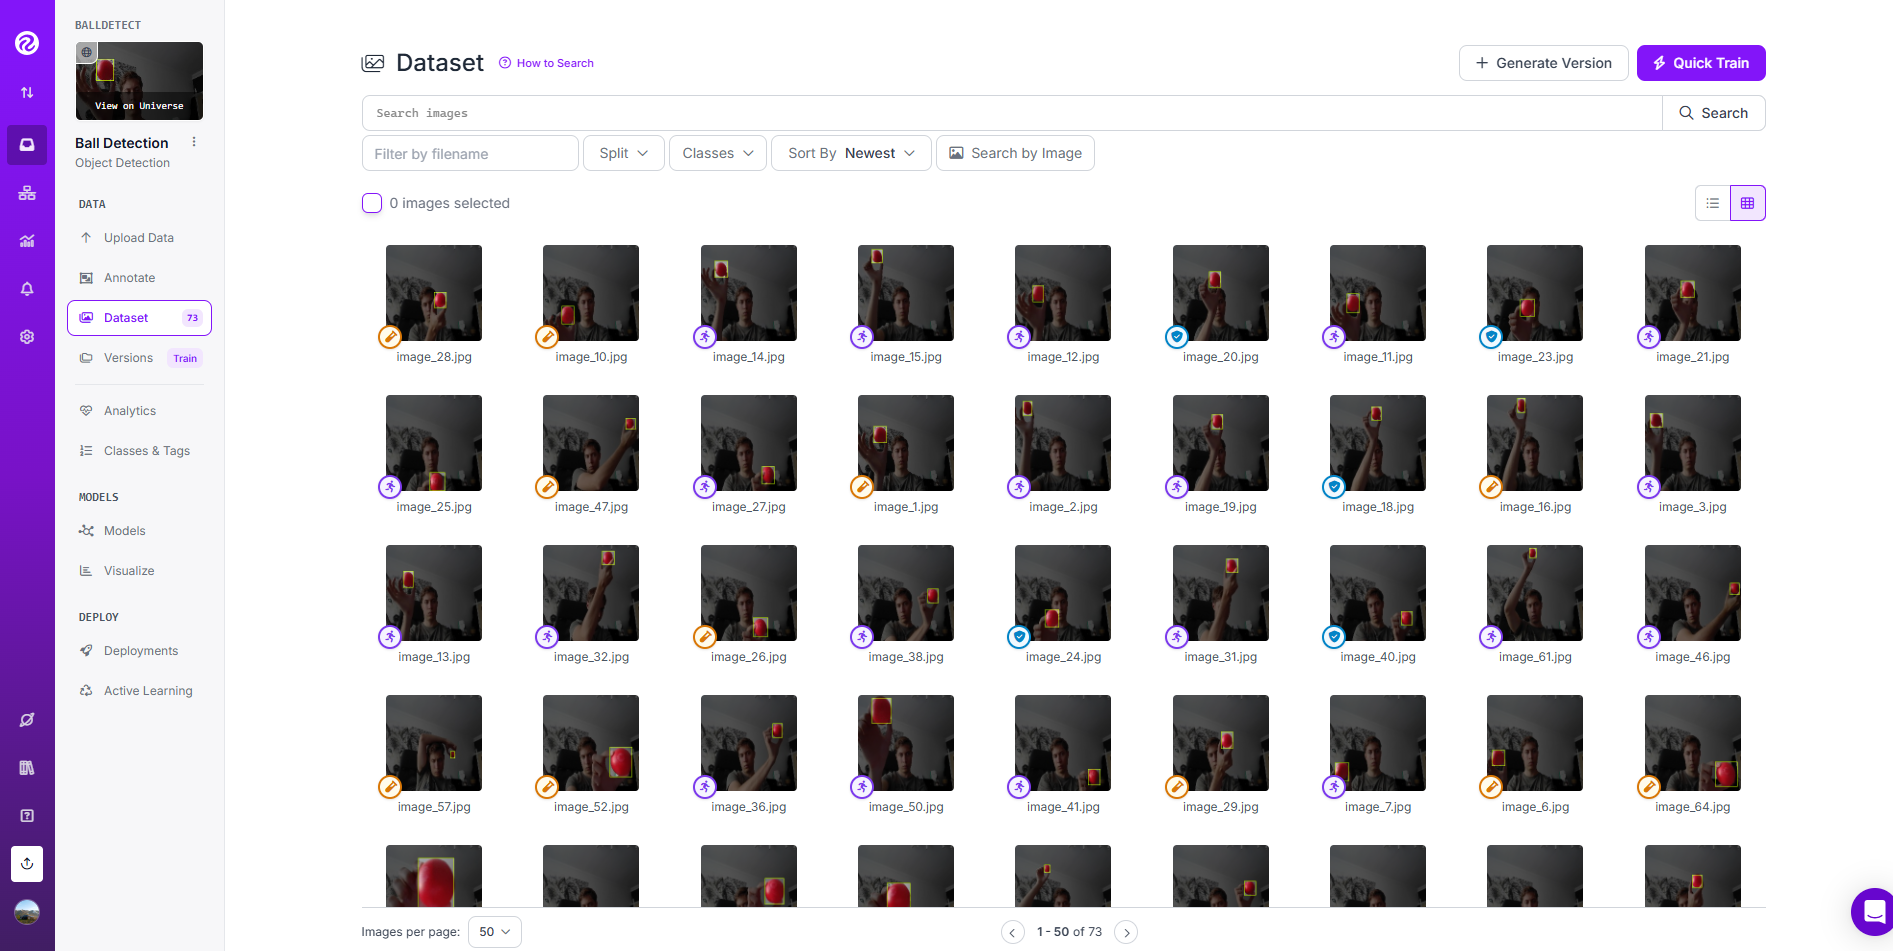
\includegraphics[width=1\textwidth]{Images/Roboflow/mainscreen.png}
	\caption{Widok strony głównej witryny Roboflow.}
	\label{fig:roboflow-main}
\end{figure}


\begin{figure}[h!]
    \centering

    \begin{subfigure}[b]{1\textwidth}
        \centering
        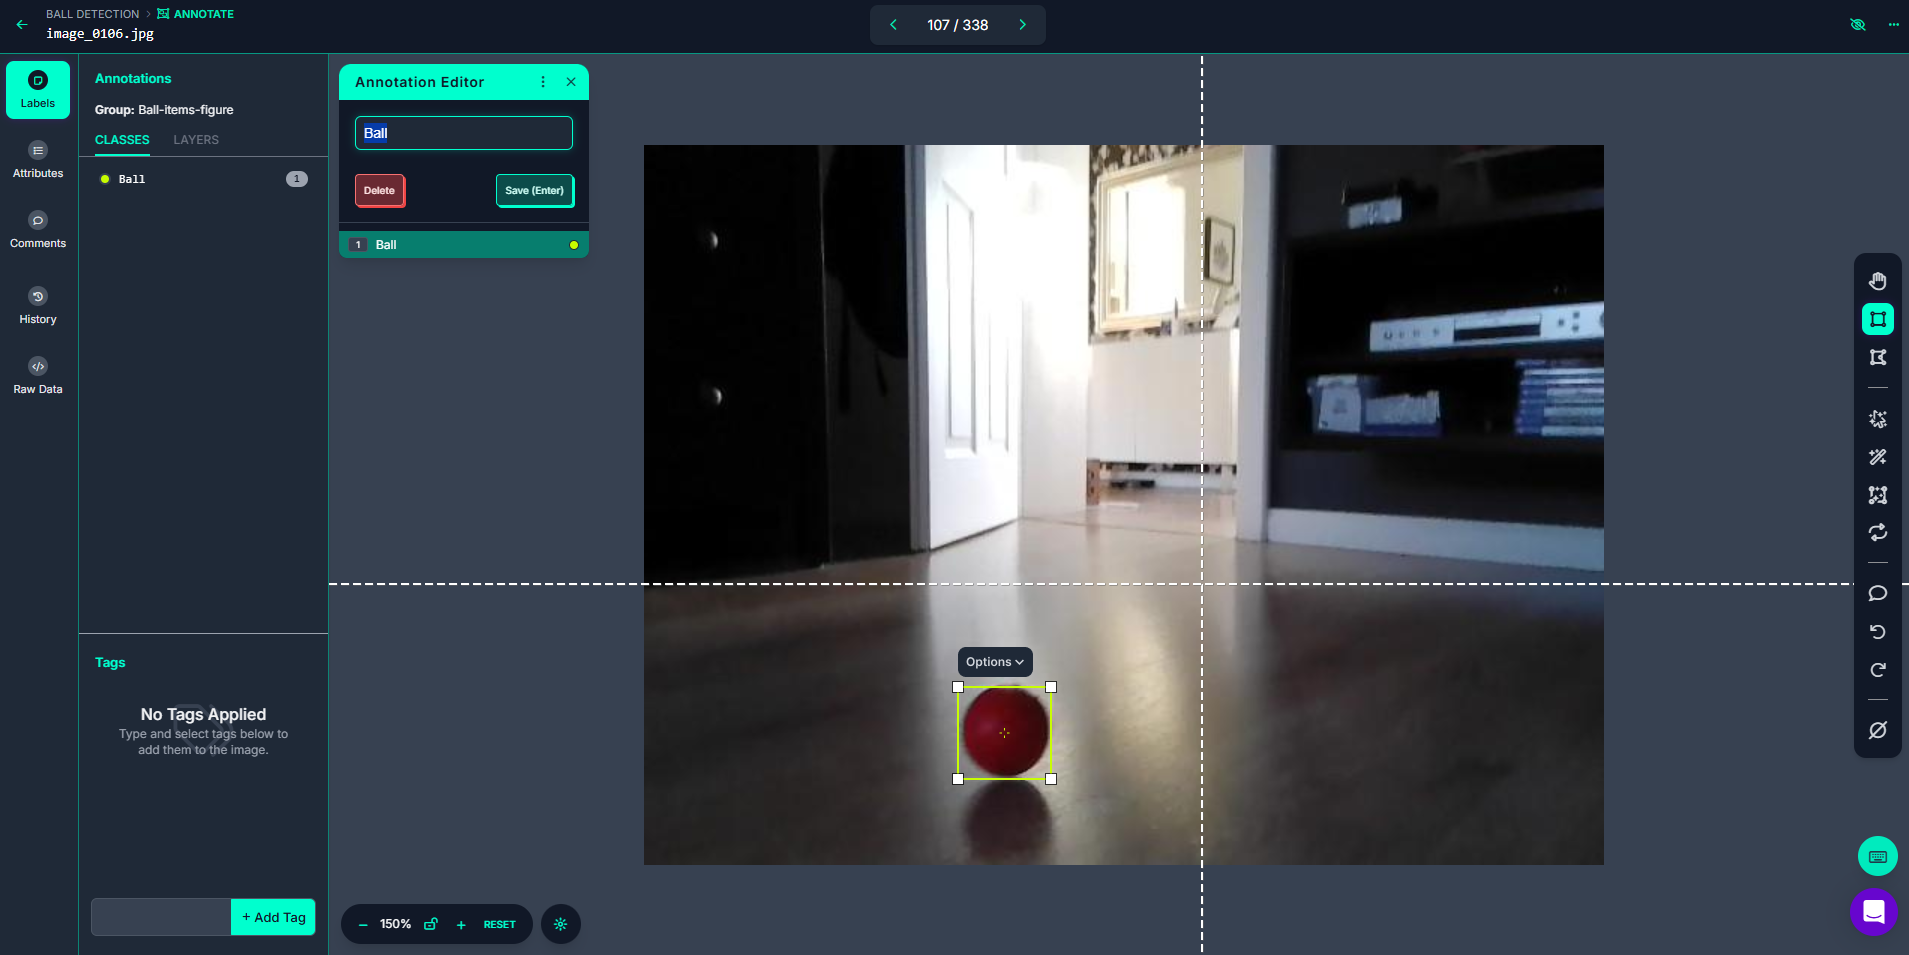
\includegraphics[width=1\textwidth]{Images/Roboflow/labeling1.png}
        \caption{Etykietowanie obiektów w Roboflow.}
        \label{fig:labeling1}
    \end{subfigure}
    
    \begin{subfigure}[b]{1\textwidth}
        \centering
        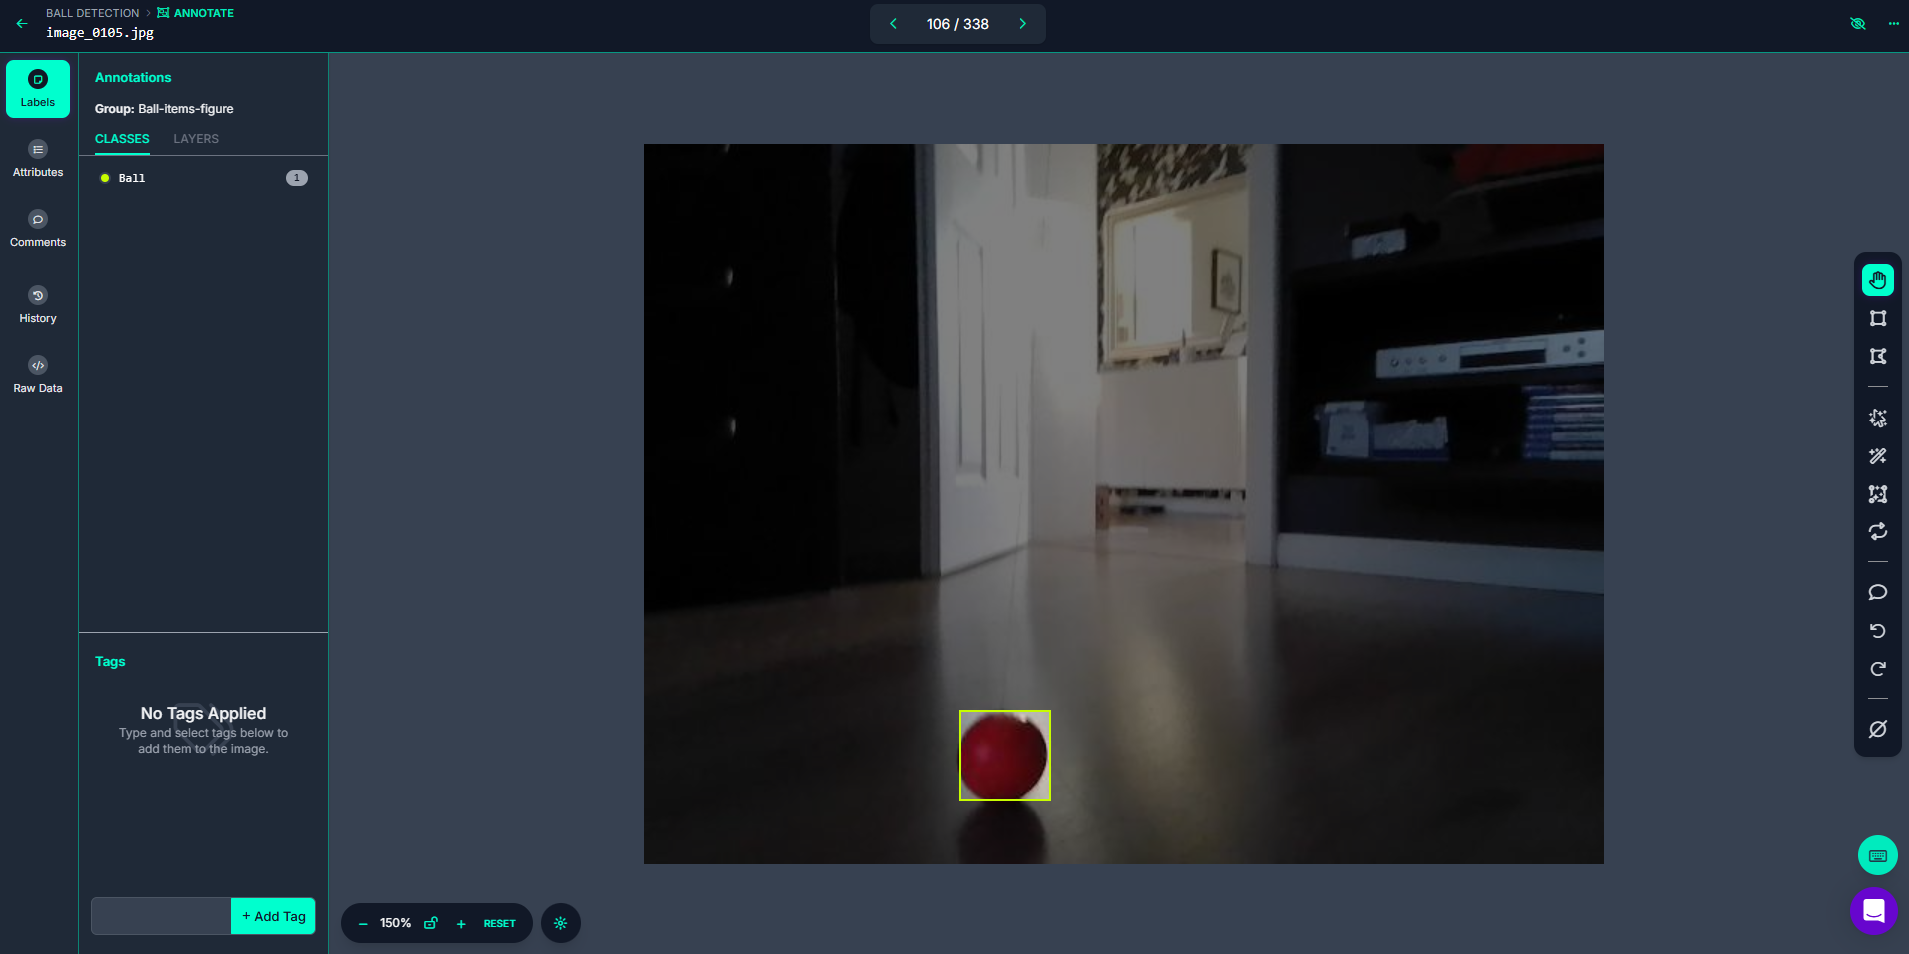
\includegraphics[width=1\textwidth]{Images/Roboflow/labeling2.png}
        \caption{Obiekt po zetykietowaniu}
        \label{fig:labeling2}
    \end{subfigure}
    
    \begin{subfigure}[b]{1\textwidth}
        \centering
        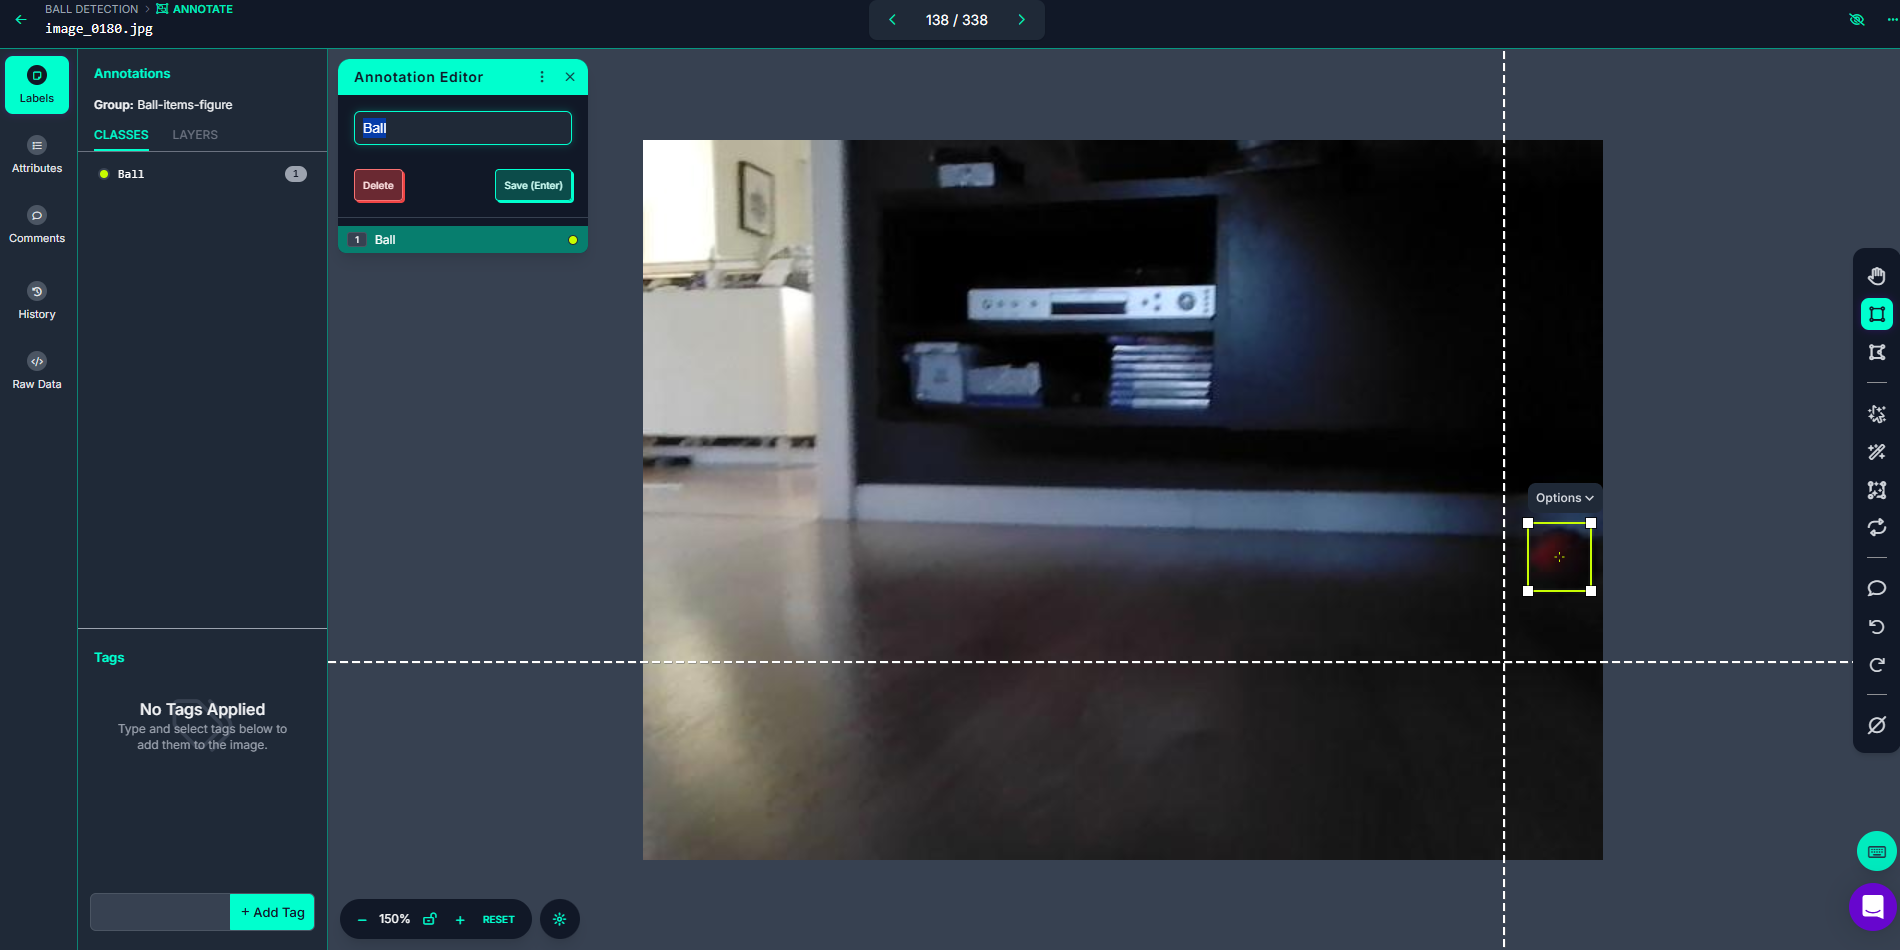
\includegraphics[width=1\textwidth]{Images/Roboflow/labeling3.png}
        \caption{Etykietowanie w słabym oświetleniu}
        \label{fig:labeling3}
    \end{subfigure}
    
    \caption{Proces użycia witryny Roboflow.}
    \label{fig:roboflow-process}
\end{figure}


\newpage
%%%% Biblioteka PyTorch %%%%%
\section{PyTorch}
PyTorch to jedna z bardziej popularnych bibliotek uczenia maszynowego, opracowanej przez Meta AI i obecnie wspieraną przez PyTorch Foundation. Biblioteka została zaprojektowana z myślą o intuicyjności, wydajności i elastyczności.

%%\paragraph{Główne cechy PyTorch}
%%\begin{itemize}
%%    \item \textbf{Dynamiczne grafy obliczeniowe}: Dzięki dynamicznemu budowaniu grafów obliczeniowych, PyTorch pozwala na elastyczne definiowanie i modyfikowanie modeli w trakcie ich działania \cite{bib:paszke2019pytorch}.
%%    \item \textbf{Obliczenia tensorowe z akceleracją GPU}: Biblioteka zapewnia wsparcie dla obliczeń tensorowych z wykorzystaniem GPU, co umożliwia szybkie przetwarzanie dużych zbiorów danych \cite{paszke2019pytorch}.
%%    \item \textbf{Wsparcie dla głębokich sieci neuronowych}: Moduł \texttt{torch.nn} ułatwia definiowanie i trenowanie złożonych modeli głębokiego uczenia.
%%\end{itemize}

\paragraph{Zastosowania PyTorch}
PyTorch jest szeroko wykorzystywany zarówno w badaniach naukowych, jak i w przemyśle. Do jego głównych zastosowań należą:
\begin{itemize}
    \item \textbf{Wizja komputerowa}: PyTorch jest wykorzystywany do trenowania modeli detekcji obiektów, takich jak YOLOv7, oraz innych architektur CNN.
    \item \textbf{Przetwarzanie języka naturalnego (NLP)}: Biblioteki takie jak Hugging Face Transformers, używane do przetwarzania języka, opierają się na PyTorch.
    \item \textbf{Autonomiczne systemy}: PyTorch znajduje zastosowanie w systemach autonomicznych, takich jak systemy nawigacji dla robotów mobilnych.
\end{itemize}

\paragraph{Społeczność i rozwój}
PyTorch posiada jedną z najbardziej aktywnych społeczności w obszarze uczenia maszynowego. Dzięki otwartemu modelowi rozwoju, społeczność regularnie wprowadza nowe funkcje, poprawki błędów oraz dedykowane narzędzia, takie jak PyTorch Lightning, które ułatwiają proces trenowania modeli.

\paragraph{Podsumowanie}
Dzięki intuicyjności, wszechstronności i wysokiej wydajności, PyTorch stał się jednym z najważniejszych narzędzi w dziedzinie głębokiego uczenia. W tej pracy PyTorch został wykorzystany jako podstawowa biblioteka do implementacji algorytmu YOLO oraz zarządzania procesami trenowania modeli.



%%%% Algorytm YOLO %%%%%
\subsection{Algorytm YOLO}
%%Algorytm YOLO (\textit{You Only Look Once}) został zaprojektowany jako zintegrowany system detekcji obiektów w czasie rzeczywistym, przekształcając problem detekcji w zadanie regresji. YOLO stosuje jedną sieć neuronową do analizy całego obrazu i równoczesnego przewidywania współrzędnych ramek ograniczających oraz klas obiektów \cite{redmon2016yolo}.

\paragraph{Założenia projektowe}
Model YOLO dzieli obraz na siatkę \( S \times S \), gdzie każda komórka siatki przewiduje:
\begin{itemize}
    \item \( B \) ramek ograniczających (\textit{bounding boxes}) wraz z ich współrzędnymi \((x, y, w, h)\),
    \item prawdopodobieństwo obecności obiektu w każdej ramce,
    \item prawdopodobieństwo klasowe dla każdego obiektu.
\end{itemize}
Łączne przewidywania są zapisywane jako tensor o wymiarze \( S \times S \times (B \cdot 5 + C) \), gdzie \( C \) to liczba klas \cite{bib:redmon_yolo}.

\paragraph{Architektura sieci YOLO}
Sieć YOLO opiera się na warstwach konwolucyjnych, w których kluczowe znaczenie ma redukcja wymiarów za pomocą warstw \( 1 \times 1 \) i \( 3 \times 3 \). W wersji YOLOv7 wprowadzono szereg usprawnień, takich jak:
\begin{itemize}
    \item użycie modułów re-parametryzowanych (\textit{re-parameterized convolution}) dla poprawy propagacji gradientu,
    \item lepsza agregacja cech w warstwach za pomocą strategii E-ELAN (\textit{Extended Efficient Layer Aggregation Networks}),
    \item optymalizacja procesu uczenia poprzez dynamiczne przypisywanie etykiet (\textit{coarse-to-fine label assignment}) \cite{bib:wang_yolov7}.
\end{itemize}

W ramach tej pracy YOLO zostało wykorzystane do detekcji obiektów w systemie wizyjnym robota mobilnego. Model YOLOv7, dzięki swojej optymalnej architekturze i wydajności, umożliwił realizację systemu wizyjnego z zachowaniem wymagań ograniczonej mocy obliczeniowej platformy Raspberry Pi.





%%%% Wymagania sprzętowe %%%%%
\section{specyfikacja techniczna}

% TODO
\chapter{[Właściwy dla kierunku -- np. Specyfikacja zewnętrzna]}
\label{ch:04}

Jeśli „Specyfikacja zewnętrzna”:
\begin{itemize}
\item  wymagania sprzętowe i programowe
\item  sposób instalacji
\item  sposób aktywacji
\item  kategorie użytkowników
\item  sposób obsługi
\item  administracja systemem
\item  kwestie bezpieczeństwa
\item  przykład działania
\item  scenariusze korzystania z systemu (ilustrowane zrzutami z ekranu lub generowanymi dokumentami)
\end{itemize}

\

%%%%%%%%%%%%%%%%%%%%%
%% RYSUNEK Z PLIKU
%
%\begin{figure}
%\centering
%
\includegraphics[width=0.5\textwidth]{./politechnika_sl_logo_bw_pion_pl.pdf}
%\caption{Podpis rysunku zawsze pod rysunkiem.}
%\label{fig:etykieta-rysunku}
%\end{figure}
%Rys. \ref{fig:etykieta-rysunku} przestawia …
%%%%%%%%%%%%%%%%%%%%%
%
%%%%%%%%%%%%%%%%%%%%%
%% WIELE RYSUNKÓW 
%
%\begin{figure}
%\centering
%\begin{subfigure}{0.4\textwidth}
%    
\includegraphics[width=\textwidth]{./politechnika_sl_logo_bw_pion_pl.pdf}
%    \caption{Lewy górny rysunek.}
%    \label{fig:lewy-gorny}
%\end{subfigure}
%\hfill
%\begin{subfigure}{0.4\textwidth}
%    
\includegraphics[width=\textwidth]{./politechnika_sl_logo_bw_pion_pl.pdf}
%    \caption{Prawy górny rysunek.}
%    \label{fig:prawy-gorny}
%\end{subfigure}
%
%\begin{subfigure}{0.4\textwidth}
%    
\includegraphics[width=\textwidth]{./politechnika_sl_logo_bw_pion_pl.pdf}
%    \caption{Lewy dolny rysunek.}
%    \label{fig:lewy-dolny}
%\end{subfigure}
%\hfill
%\begin{subfigure}{0.4\textwidth}
%    
\includegraphics[width=\textwidth]{./politechnika_sl_logo_bw_pion_pl.pdf}
%    \caption{Prawy dolny rysunek.}
%    \label{fig:prawy-dolny}
%\end{subfigure}
%        
%\caption{Wspólny podpis kilku rysunków.}
%\label{fig:wiele-rysunkow}
%\end{figure}
%Rys. \ref{fig:wiele-rysunkow} przestawia wiele ważnych informacji, np. rys. \ref{fig:prawy-gorny} jest na prawo u góry.
%%%%%%%%%%%%%%%%%%%%%


 
\begin{figure}
\centering
\begin{tikzpicture}
\begin{axis}[
    y tick label style={
        /pgf/number format/.cd,
            fixed,   % po zakomentowaniu os rzednych jest indeksowana wykladniczo
            fixed zerofill, % 1.0 zamiast 1
            precision=1,
        /tikz/.cd
    },
    x tick label style={
        /pgf/number format/.cd,
            fixed,
            fixed zerofill,
            precision=2,
        /tikz/.cd
    }
]
\addplot [domain=0.0:0.1] {rnd};
\end{axis} 
\end{tikzpicture}
\caption{Podpis rysunku po rysunkiem.}
\label{fig:2}
\end{figure}



% TODO
\chapter{[Właściwy dla kierunku -- np. Specyfikacja wewnętrzna]}
\label{ch:05}


Jeśli „Specyfikacja wewnętrzna”:
\begin{itemize}
\item przedstawienie idei
\item architektura systemu
\item opis struktur danych (i organizacji baz danych)
\item komponenty, moduły, biblioteki, przegląd ważniejszych klas (jeśli występują)
\item przegląd ważniejszych algorytmów (jeśli występują)
\item szczegóły implementacji wybranych fragmentów, zastosowane wzorce projektowe
\item diagramy UML
\end{itemize}

% % % % % % % % % % % % % % % % % % % % % % % % % % % % % % % % % % % 
% Pakiet minted wymaga importu: \usepackage{minted}                 %
% i specjalnego kompilowania:                                       %
% pdflatex -shell-escape main                                       %
% % % % % % % % % % % % % % % % % % % % % % % % % % % % % % % % % % % 


Krótka wstawka kodu w linii tekstu jest możliwa, np.  \lstinline|int a;| (biblioteka \texttt{listings})% lub  \mintinline{C++}|int a;| (biblioteka \texttt{minted})
. 
Dłuższe fragmenty lepiej jest umieszczać jako rysunek, np. kod na rys \ref{fig:pseudokod:listings}% i rys. \ref{fig:pseudokod:minted}
, a naprawdę długie fragmenty – w załączniku.


\begin{figure}
\centering
\begin{lstlisting}
class test : public basic
{
    public:
      test (int a);
      friend std::ostream operator<<(std::ostream & s, 
                                     const test & t);
    protected:
      int _a;  
      
};
\end{lstlisting}
\caption{Pseudokod w \texttt{listings}.}
\label{fig:pseudokod:listings}
\end{figure}

%\begin{figure}
%\centering
%\begin{minted}[linenos,frame=lines]{c++}
%class test : public basic
%{
%    public:
%      test (int a);
%      friend std::ostream operator<<(std::ostream & s, 
%                                     const test & t);
%    protected:
%      int _a;  
%      
%};
%\end{minted}
%\caption{Pseudokod w \texttt{minted}.}
%\label{fig:pseudokod:minted}
%\end{figure}




% TODO
\chapter{Weryfikacja i walidacja}
\label{ch:06}
\begin{itemize}
\item sposób testowania w ramach pracy (np. odniesienie do modelu V)
\item organizacja eksperymentów
\item przypadki testowe zakres testowania (pełny/niepełny)
\item wykryte i usunięte błędy
\item opcjonalnie wyniki badań eksperymentalnych
\end{itemize}

\begin{table}
\centering
\caption{Nagłówek tabeli jest nad tabelą.}
\label{id:tab:wyniki}
\begin{tabular}{rrrrrrrr}
\toprule
	         &                                     \multicolumn{7}{c}{metoda}                                      \\
	         \cmidrule{2-8}
	         &         &         &        \multicolumn{3}{c}{alg. 3}        & \multicolumn{2}{c}{alg. 4, $\gamma = 2$} \\
	         \cmidrule(r){4-6}\cmidrule(r){7-8}
	$\zeta$ &     alg. 1 &   alg. 2 & $\alpha= 1.5$ & $\alpha= 2$ & $\alpha= 3$ &   $\beta = 0.1$  &   $\beta = -0.1$ \\
\midrule
	       0 &  8.3250 & 1.45305 &       7.5791 &    14.8517 &    20.0028 & 1.16396 &                       1.1365 \\
	       5 &  0.6111 & 2.27126 &       6.9952 &    13.8560 &    18.6064 & 1.18659 &                       1.1630 \\
	      10 & 11.6126 & 2.69218 &       6.2520 &    12.5202 &    16.8278 & 1.23180 &                       1.2045 \\
	      15 &  0.5665 & 2.95046 &       5.7753 &    11.4588 &    15.4837 & 1.25131 &                       1.2614 \\
	      20 & 15.8728 & 3.07225 &       5.3071 &    10.3935 &    13.8738 & 1.25307 &                       1.2217 \\
	      25 &  0.9791 & 3.19034 &       5.4575 &     9.9533 &    13.0721 & 1.27104 &                       1.2640 \\
	      30 &  2.0228 & 3.27474 &       5.7461 &     9.7164 &    12.2637 & 1.33404 &                       1.3209 \\
	      35 & 13.4210 & 3.36086 &       6.6735 &    10.0442 &    12.0270 & 1.35385 &                       1.3059 \\
	      40 & 13.2226 & 3.36420 &       7.7248 &    10.4495 &    12.0379 & 1.34919 &                       1.2768 \\
	      45 & 12.8445 & 3.47436 &       8.5539 &    10.8552 &    12.2773 & 1.42303 &                       1.4362 \\
	      50 & 12.9245 & 3.58228 &       9.2702 &    11.2183 &    12.3990 & 1.40922 &                       1.3724 \\
\bottomrule
\end{tabular}
\end{table}  



% TODO
\chapter{Podsumowanie i wnioski}
\begin{itemize}
\item uzyskane wyniki w świetle postawionych celów i zdefiniowanych wyżej wymagań
\item kierunki ewentualnych danych prac (rozbudowa funkcjonalna …)
\item problemy napotkane w trakcie pracy
\end{itemize}



\backmatter

%\bibliographystyle{plplain}  % bibtex
%\bibliography{biblio} % bibtex
\printbibliography           % biblatex
\addcontentsline{toc}{chapter}{Bibliografia}

\begin{appendices}

% TODO
\chapter{Spis skrótów i symboli}

\begin{itemize}
\item[DNA] kwas deoksyrybonukleinowy (ang. \english{deoxyribonucleic acid})
\item[MVC] model -- widok -- kontroler (ang. \english{model--view--controller}) 
\item[$N$] liczebność zbioru danych
\item[$\mu$] stopnień przyleżności do zbioru
\item[$\mathbb{E}$] zbiór krawędzi grafu
\item[$\mathcal{L}$] transformata Laplace'a 
\end{itemize}


% TODO
\chapter{Źródła}

Jeżeli w pracy konieczne jest umieszczenie długich fragmentów kodu źródłowego, należy je przenieść w to miejsce.

\begin{lstlisting}
if (_nClusters < 1)
	throw std::string ("unknown number of clusters");
if (_nIterations < 1 and _epsilon < 0)
	throw std::string ("You should set a maximal number of iteration or minimal difference -- epsilon.");
if (_nIterations > 0 and _epsilon > 0)
	throw std::string ("Both number of iterations and minimal epsilon set -- you should set either number of iterations or minimal epsilon.");
\end{lstlisting}


% % % % % % % % % % % % % % % % % % % % % % % % % % % % % % % % % % % 
% Pakiet minted wymaga odkomentowania w pliku config/settings.tex   %
% importu pakietu minted: \usepackage{minted}                       %
% i specjalnego kompilowania:                                       %
% pdflatex -shell-escape praca                                      %
% % % % % % % % % % % % % % % % % % % % % % % % % % % % % % % % % % % 

%\begin{minted}[linenos,breaklines,frame=lines]{c++}
%if (_nClusters < 1)
%   throw std::string ("unknown number of clusters");
%if (_nIterations < 1 and _epsilon < 0)
%   throw std::string ("You should set a maximal number of iteration or minimal difference -- epsilon.");
%if (_nIterations > 0 and _epsilon > 0)
%   throw std::string ("Both number of iterations and minimal epsilon set -- you should set either number of iterations or minimal epsilon.");
%\end{minted}


% TODO
\chapter{Lista dodatkowych plików, uzupełniających tekst pracy} 


W systemie do pracy dołączono dodatkowe pliki zawierające:
\begin{itemize}
\item źródła programu,
\item dane testowe,
\item film pokazujący działanie opracowanego oprogramowania lub zaprojektowanego i~wykonanego urządzenia,
\item itp.
\end{itemize}


\listoffigures
\addcontentsline{toc}{chapter}{Spis rysunków}
\listoftables
\addcontentsline{toc}{chapter}{Spis tabel}

\end{appendices}

\end{document}


%% Finis coronat opus.

